% SIAM Article Template
\documentclass[review,onefignum,onetabnum]{siamart171218}
\usepackage{amssymb}
\usepackage{graphicx}
\graphicspath{ {./} }
% Information that is shared between the article and the supplement
% (title and author information, macros, packages, etc.) goes into
% ex_shared.tex. If there is no supplement, this file can be included
% directly.

% SIAM Shared Information Template
% This is information that is shared between the main document and any
% supplement. If no supplement is required, then this information can
% be included directly in the main document.


% Packages and macros go here
\usepackage{lipsum}
\usepackage{amsfonts}
\usepackage{graphicx}
\usepackage{epstopdf}
\usepackage{algorithmic}
\ifpdf
  \DeclareGraphicsExtensions{.eps,.pdf,.png,.jpg}
\else
  \DeclareGraphicsExtensions{.eps}
\fi

% Add a serial/Oxford comma by default.
\newcommand{\creflastconjunction}{, and~}

% Used for creating new theorem and remark environments
\newsiamremark{remark}{Remark}
\newsiamremark{hypothesis}{Hypothesis}
\crefname{hypothesis}{Hypothesis}{Hypotheses}
\newsiamthm{claim}{Claim}

% Sets running headers as well as PDF title and authors
\headers{Movie Recommendation}{N. Grant, R. Guin, T. Hom, S. Qiu}

% Title. If the supplement option is on, then "Supplementary Material"
% is automatically inserted before the title.
\title{Movie Recommendation}

% Authors: full names plus addresses.
\author{Nathan Grant
\and Rudra Guin
\and Tyler Hom
\and Steven Qiu}
  
\usepackage{amsopn}
\DeclareMathOperator{\diag}{diag}


%%% Local Variables: 
%%% mode:latex
%%% TeX-master: "ex_article"
%%% End: 


% Optional PDF information
\ifpdf
\hypersetup{
  pdftitle={Movie Recommendation},
  pdfauthor={N. Grant, R. Guin, T. Hom, S. Qiu}
}
\fi

% The next statement enables references to information in the
% supplement. See the xr-hyperref package for details.

\externaldocument{ex_supplement}


\begin{document}

\maketitle

% REQUIRED
\begin{abstract}
In this project we explored various techniques, both used in and out of class to try to accurately predict movie ratings based off of the data set used in lab. Using both techniques used in  and out of class, we used algorithms which performed far better than random on test data. Movie reccomendaitions made on given users were also accurate, most times getting the users genre preferences right.
\end{abstract}

% REQUIRED
\begin{keywords}
  Movie Recommendation, Decision Trees, SVD
\end{keywords}

% REQUIRED
\begin{AMS}
  15A18, 62P20
\end{AMS}

\section{Introduction}
Recommendation systems are some of the most important applications in modern day machine learning. Companies such as Amazon must use purchase history and search trends to predict which items you might want to buy. Netflix faces a similar dilemma in that users will watch and rate movies and they must recommend new movies which the users will like. In this project we explored many approaches to movie recommendation to see what offered the best results.

The biggest challenge to recommendation systems is the sparsity to the data. In the data set any given user only rates a small fraction of the total of movies in the database. Such sparse information makes it hard to make very accurate predictions about what movies the users would enjoy. 

	We evaluate our results based off of two metrics, accuracy of the classification of a users movie rating, and the mean absolute deviation from the correct rating.

\section{Methods}
\label{sec:methods}
The movie recommendation system was evaluated in one of two ways. One way is through human evaluation of the results. Given a user and their rated movies, the algorithm could output movies that they might like. However, this gets tricky because there is no metric to evaluate how good these recommendations actually are. The second option is to take out examples from the training data to use them as test data which was the most promising option. First, we approached the problem using classification models where a users data would be input along with the movie data in order to predict what the user would rate the movie. 

	Our first approach was to use decision trees. These techniques resulted in accuracies which were not much better than random. Due to the sparsity of the data, it is very hard for a single movie to impact the information gain of a tree split. This results in trees which are very deep and are split on attributes which do not change the distribution of the predicted classes much if at all. We moved onto random forests and gradient boosted trees which did not increase predictive power much, if at all, because the problem isn't particularly suited for those models. The tree splits based off of whether things are greater than or less than a certain value but entropy would increase more if it was just equal to or not equal to instead.  
	
	Next we used neural networks to try to predict movie rating. This method also didn't work too well because of two reasons, the sparsity of the problem, and the lack of data. Neural nets require a large amount of data to be able to make good predictions and in the data set there were only 3000 different users, and some users rated only one movie. This sparsity and lack of data makes it hard for neural nets to make good ratings. 
	
	Afterwards we tried the method of alternating least squares. We used the table where the columns were movie ratings and teh rows were users. This method uses matrix factorization to split the users/ratings table into two smaller tables, which can then be used to determine what a user would rate any given movie. This method uses gradient descent to approximate the two matrices which makes computation much faster.
	
	Finally we tried the approach of using SVD and then using KNN to chose movie rating. The initial appeal to the SVD method is the fact that it reduces the high dimensional sparse ratings vector down to a n-dimensional dense vector which we can assume to be some representation of the users preferences. To predict what the user will rate a given movie uses a varying KNN approach. Given some movieID M , user U and actual rating R, the model pulls up the user U's rating vector used for the SVD (the test set). Then it will alter the value for movie M with values 1-5 and then pass it through the SVD model. So 5 dense vectors are returned which are then compared to the test user point by elucidian distance. Whichever point is the closest is chosen as the user U's rating R for movie M. 

\begin{algorithm}
\caption{SVD Nearest Weighted Neighbors}
\begin{algorithmic}
\STATE{Define Epochs: ${1-N}$}
\WHILE{$n < Epochs$}
\STATE{Predict nearest neighbors}
\STATE{Compute error E using squared error of predictions}
\STATE{Find $ \triangledown {E = (\frac{\delta E}{\delta W_{i}},...\frac{\delta E}{\delta w_{comp}})}$}
\STATE{Update $W := -\gamma*\triangledown E$ }
\STATE{Update $W :=  (\sum_{}^{} W_{i} )^{-1}}*W $}
\STATE{$n += 1$}

\ENDWHILE
\RETURN $W$
\end{algorithmic}
\end{algorithm}

The technique was improved on by using a weighted distance instead. The held out test points were split up into two parts , two-thirds of the points were reserved for computing the gradient of the loss and the last third was used to actually test the accuracy of the model. The same technique still held where the closest point would be picked greedily as the classification. To compute the gradient, we need to know what the actual class is in order to compute an error from the predicted class. This time we compute the compressed vector for both the predicted rating and the actual rating of the movie. We then compute the error between these two vectors and then use it as the gradient vector for the weights. After repeating this process 1000's of times the result is a set of weights which marginally increases prediction accuracy, and reduces variance.

\section{Results}
\label{sec:results}

The regression tree method resulted in an MAD of .8938 using 10-cross-fold-validation which meant that the predictions would not have been that good. The Random Forest Regression Tree barely performed any better with a MAD of .8936. This is to be expected because its just an ensamble of already poor performing decision trees. The Gradient Bootsed Tree also perfoemed simmarly to the Decision Tree with an MAD of .8938. We were expecting it to perform slightly better than the other tree methods because of its error correcting nature on misclassified points, however it failed to meet expectations. The Neural Netwoek Regressor had a slight performance increase over the other methods with an MAD of .8799. However, the neural net didn't have enough data to be able to generalize. This technique should be pursued when more data is available. The alternating least squares method performed even better with a MAD of .8685. Again given more data this approach would perform even better. The SVD with varying KNN method acheived an MAD of .6326. This exceeded expectations and perfmrmed signifiantly better than the other methods. Its not entirely clear how this method would scale with more data. The SVD with Weighted Varying KNN performed the best with an MAD of .4838. This method was sensitive to initial conditions, however when set right, performed well. Below is an image showing the reccomendations that the SVD method returns and table of all of our collected data respectivley.
\begin{figure}[H]
  \centering
    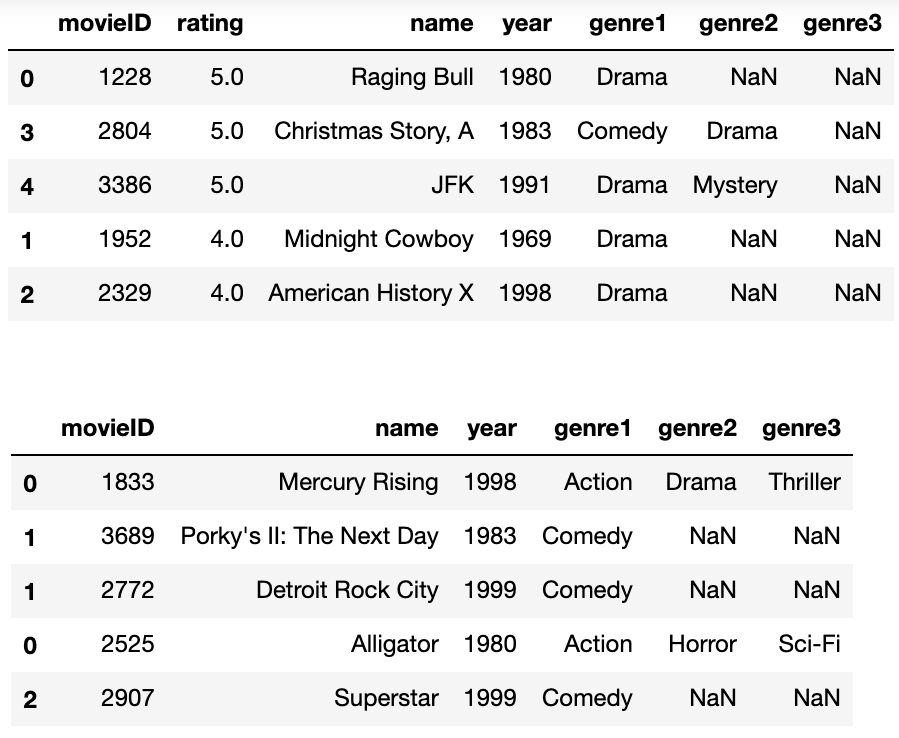
\includegraphics[width=14cm, height=11.5cm]{reccomendations}
  \caption{Top table preferences, Bottom table reccomendations}
  \label{fig:reccomendations}
\end{figure}
\begin{table}[H]
\centering
\caption {MAD of Methods Used} \label{tab:title} 
\begin{tabular}{|l|l|}
\hline
Method Used & MAD \\ \hline
Regression Tree               & 0.8938 \\ \hline
Gradient Boosted Tree         & 0.8938 \\ \hline
Random Forest                 & 0.8936 \\ \hline
Neural Network                & 0.8799 \\ \hline
Alternating Least Squares         & 0.8685 \\ \hline
SVD  with Varying KNN         & 0.6326 \\ \hline
SVD with Weighted Varying KNN & 0.4838\\ \hline
\end{tabular}
\end{table}

Top table is the user who the algorithm is to reccomend movies to.
Bottom table is the reccomended movies. As you can see the results match up pretty well according to genre.

\section{Summary}
\label{sec:summary}

The drawback to some of these techniques, especially the gradient SVD method, is the time it takes to compute. Because of this it would be infeasable to use in practice as an actual movie reccomendation system. Overall it is particularly interesting that the KNN implemenation worked so well. However, its performance was in some cases heavily impacted by the initial conditions. For example, the SVD could have initialized in a favorible state for the test set, resulting in higher accuracy. The gradient method helped reduce the variance in outcomes significantly given that weights are all initialized to 1. If initialized otherwise, it adds another element of variance in model outcomes.

Further studies would probably be most interested in the Alternating Least Squares approach. It isn't as computationlly intensive and it's the technique used in industry. Further implementations could include low rank approximation to capture the spread and use the spectral norm to automatically regularize and adjust rank. In industry, if there is a plentiful amount of data, neural networks can be utilized to create the factorized matricies and increase predictive accuracy.

Given a lot of data, reinforcement learning could also be a worthwile aproach. This would work by giving the recommendation system a reward each time that it predicts a users actions correctly. This implementaion would take a lot of data to work effectivley so it wasn't feasable for this particular data set. 
\end{document}
